

\tikzset{every picture/.style={line width=0.75pt}} %set default line width to 0.75pt        
\begin{center}
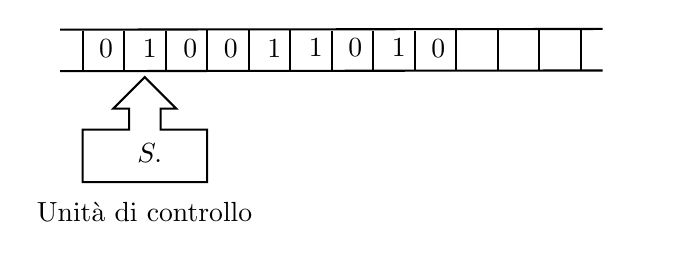
\begin{tikzpicture}[x=0.75pt,y=0.75pt,yscale=-1,xscale=1]
%uncomment if require: \path (0,300); %set diagram left start at 0, and has height of 300

%Straight Lines [id:da7275362281558355] 
\draw    (189.33,120) -- (450.67,119.67) ;


%Straight Lines [id:da29120625547318935] 
\draw    (189.33,140) -- (450.67,139.67) ;


%Straight Lines [id:da7625664285601652] 
\draw    (200.25,120.5) -- (200.25,140) ;


%Straight Lines [id:da10240131930295271] 
\draw    (220.25,120.5) -- (220.25,140) ;


%Straight Lines [id:da978604948835289] 
\draw    (240.25,120.5) -- (240.25,140) ;


%Straight Lines [id:da9959379734940303] 
\draw    (260.25,120) -- (260.25,139.5) ;


%Straight Lines [id:da9581700306481775] 
\draw    (280.25,120) -- (280.25,139.5) ;


%Straight Lines [id:da4437031266260554] 
\draw    (300.25,120) -- (300.25,139.5) ;


%Straight Lines [id:da6017637495165318] 
\draw    (320.25,120.5) -- (320.25,140) ;


%Straight Lines [id:da5089858317275813] 
\draw    (340.25,120.5) -- (340.25,140) ;


%Straight Lines [id:da043107959414806274] 
\draw    (360.25,120.5) -- (360.25,140) ;


%Straight Lines [id:da724113904491829] 
\draw    (380.25,120) -- (380.25,139.5) ;


%Straight Lines [id:da049275772796910644] 
\draw    (400.25,120) -- (400.25,139.5) ;


%Straight Lines [id:da6822986153958353] 
\draw    (420.25,120) -- (420.25,139.5) ;


%Straight Lines [id:da0016020051178489148] 
\draw    (440.25,120) -- (440.25,139.5) ;


%Callout Right Arrow [id:dp576862285756073] 
\draw   (200.13,193.5) -- (200.13,168.19) -- (222.53,168.19) -- (222.53,158.06) -- (214.94,158.06) -- (230.13,142.88) -- (245.31,158.06) -- (237.72,158.06) -- (237.72,168.19) -- (260.13,168.19) -- (260.13,193.5) -- cycle ;

% Text Node
\draw (211.5,129) node   {$0$};
% Text Node
\draw (232.5,129) node   {$1$};
% Text Node
\draw (252,129) node   {$0$};
% Text Node
\draw (271.5,129) node   {$0$};
% Text Node
\draw (292.5,129) node   {$1$};
% Text Node
\draw (312.5,128.5) node   {$1$};
% Text Node
\draw (331.5,128.5) node   {$0$};
% Text Node
\draw (473,123.5) node   {$\dotsc $};
% Text Node
\draw (232.5,179.5) node   {$S.$};
% Text Node
\draw (230,208) node  [align=left] {Unità di controllo};
% Text Node
\draw (352.5,128.5) node   {$1$};
% Text Node
\draw (371.5,129) node   {$0$};


\end{tikzpicture}
\end{center}